\documentclass{standalone}
\usepackage{tikz}
\usetikzlibrary{patterns, positioning}

\begin{document}
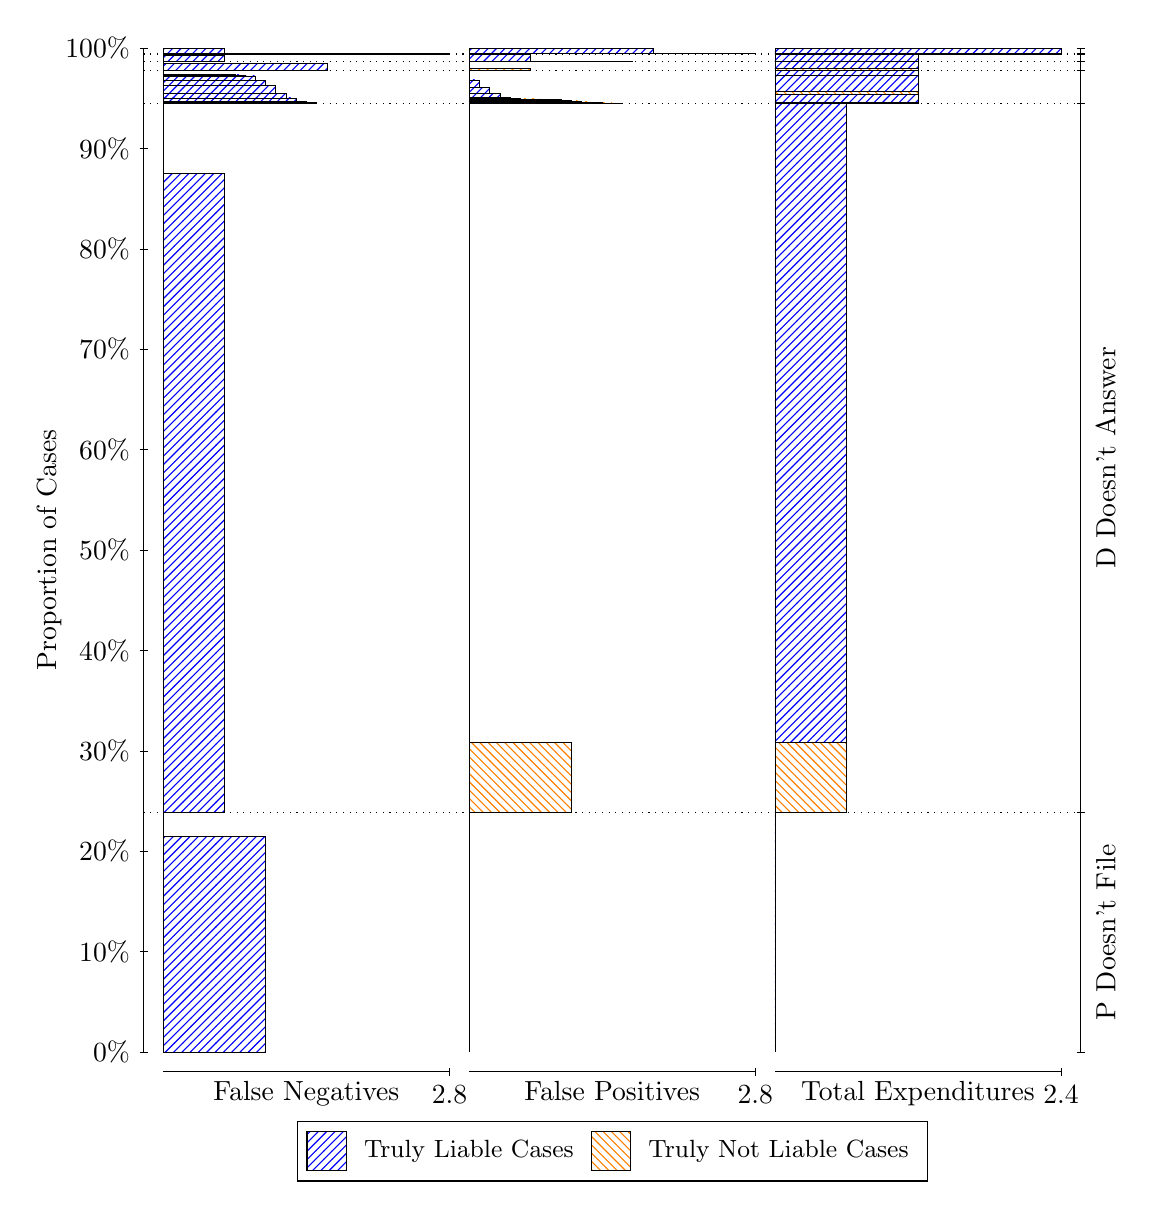
\begin{tikzpicture}
\draw[black, very thin] (1.5,1.75) -- (1.5,14.5);
\node[rotate=90, anchor=center] at (0.3, 8.125) {Proportion of Cases};
\draw[black, very thin] (1.45,1.75) -- (1.55,1.75);
\node[anchor=east] at (1.45, 1.75) {0\%};
\draw[black, very thin] (1.45,3.025) -- (1.55,3.025);
\node[anchor=east] at (1.45, 3.025) {10\%};
\draw[black, very thin] (1.45,4.3) -- (1.55,4.3);
\node[anchor=east] at (1.45, 4.3) {20\%};
\draw[black, very thin] (1.45,5.575) -- (1.55,5.575);
\node[anchor=east] at (1.45, 5.575) {30\%};
\draw[black, very thin] (1.45,6.85) -- (1.55,6.85);
\node[anchor=east] at (1.45, 6.85) {40\%};
\draw[black, very thin] (1.45,8.125) -- (1.55,8.125);
\node[anchor=east] at (1.45, 8.125) {50\%};
\draw[black, very thin] (1.45,9.4) -- (1.55,9.4);
\node[anchor=east] at (1.45, 9.4) {60\%};
\draw[black, very thin] (1.45,10.675) -- (1.55,10.675);
\node[anchor=east] at (1.45, 10.675) {70\%};
\draw[black, very thin] (1.45,11.95) -- (1.55,11.95);
\node[anchor=east] at (1.45, 11.95) {80\%};
\draw[black, very thin] (1.45,13.225) -- (1.55,13.225);
\node[anchor=east] at (1.45, 13.225) {90\%};
\draw[black, very thin] (1.45,14.5) -- (1.55,14.5);
\node[anchor=east] at (1.45, 14.5) {100\%};

\draw[black, very thin] (13.4,1.75) -- (13.4,14.5);
\draw[black, very thin] (13.35,1.75) -- (13.45,1.75);
\node[anchor=west] at (13.35, 1.75) {};
\draw[black, very thin] (13.35,4.7921) -- (13.45,4.7921);
\node[anchor=west] at (13.35, 4.7921) {};
\draw[black, very thin] (13.35,13.8) -- (13.45,13.8);
\node[anchor=west] at (13.35, 13.8) {};
\draw[black, very thin] (13.35,14.22) -- (13.45,14.22);
\node[anchor=west] at (13.35, 14.22) {};
\draw[black, very thin] (13.35,14.328) -- (13.45,14.328);
\node[anchor=west] at (13.35, 14.328) {};
\draw[black, very thin] (13.35,14.415) -- (13.45,14.415);
\node[anchor=west] at (13.35, 14.415) {};
\draw[black, very thin] (13.35,14.43) -- (13.45,14.43);
\node[anchor=west] at (13.35, 14.43) {};
\draw[black, very thin] (13.35,14.5) -- (13.45,14.5);
\node[anchor=west] at (13.35, 14.5) {};

\draw[black, very thin, pattern color=blue, pattern=north east lines] (1.75,1.75) rectangle (3.0476,4.4879);
\draw[black, very thin, pattern color=orange, pattern=north west lines] (1.75,4.4879) rectangle (1.75,4.7921);
\draw[black, very thin, pattern color=blue, pattern=north east lines] (1.75,4.7921) rectangle (2.5286,12.912);
\draw[black, very thin, pattern color=orange, pattern=north west lines] (1.75,12.912) rectangle (1.75,13.8);
\draw[black, very thin, pattern color=blue, pattern=north east lines] (1.75,13.8) rectangle (3.6964,13.812);
\draw[black, very thin, pattern color=blue, pattern=north east lines] (1.75,13.812) rectangle (3.5667,13.82);
\draw[black, very thin, pattern color=blue, pattern=north east lines] (1.75,13.82) rectangle (3.4369,13.868);
\draw[black, very thin, pattern color=blue, pattern=north east lines] (1.75,13.868) rectangle (3.3071,13.924);
\draw[black, very thin, pattern color=blue, pattern=north east lines] (1.75,13.924) rectangle (3.1774,14.023);
\draw[black, very thin, pattern color=blue, pattern=north east lines] (1.75,14.023) rectangle (3.0476,14.093);
\draw[black, very thin, pattern color=blue, pattern=north east lines] (1.75,14.093) rectangle (2.9179,14.145);
\draw[black, very thin, pattern color=blue, pattern=north east lines] (1.75,14.145) rectangle (2.7881,14.159);
\draw[black, very thin, pattern color=blue, pattern=north east lines] (1.75,14.159) rectangle (2.6583,14.167);
\draw[black, very thin, pattern color=orange, pattern=north west lines] (1.75,14.167) rectangle (1.75,14.22);
\draw[black, very thin, pattern color=blue, pattern=north east lines] (1.75,14.22) rectangle (3.8262,14.309);
\draw[black, very thin, pattern color=orange, pattern=north west lines] (1.75,14.309) rectangle (1.75,14.328);
\draw[black, very thin, pattern color=blue, pattern=north east lines] (1.75,14.328) rectangle (2.5286,14.409);
\draw[black, very thin, pattern color=orange, pattern=north west lines] (1.75,14.409) rectangle (1.75,14.415);
\draw[black, very thin, pattern color=blue, pattern=north east lines] (1.75,14.415) rectangle (5.3833,14.427);
\draw[black, very thin, pattern color=orange, pattern=north west lines] (1.75,14.427) rectangle (1.75,14.43);
\draw[black, very thin, pattern color=blue, pattern=north east lines] (1.75,14.43) rectangle (2.5286,14.499);
\draw[black, very thin, pattern color=orange, pattern=north west lines] (1.75,14.499) rectangle (1.75,14.5);
\draw[black, very thin, pattern color=orange, pattern=north west lines] (5.6333,1.75) rectangle (5.6333,2.0542);
\draw[black, very thin, pattern color=blue, pattern=north east lines] (5.6333,2.0542) rectangle (5.6333,4.7921);
\draw[black, very thin, pattern color=orange, pattern=north west lines] (5.6333,4.7921) rectangle (6.931,5.6797);
\draw[black, very thin, pattern color=blue, pattern=north east lines] (5.6333,5.6797) rectangle (5.6333,13.8);
\draw[black, very thin, pattern color=orange, pattern=north west lines] (5.6333,13.8) rectangle (7.5798,13.801);
\draw[black, very thin, pattern color=orange, pattern=north west lines] (5.6333,13.801) rectangle (7.45,13.802);
\draw[black, very thin, pattern color=orange, pattern=north west lines] (5.6333,13.802) rectangle (7.3202,13.806);
\draw[black, very thin, pattern color=orange, pattern=north west lines] (5.6333,13.806) rectangle (7.1905,13.817);
\draw[black, very thin, pattern color=orange, pattern=north west lines] (5.6333,13.817) rectangle (7.0607,13.83);
\draw[black, very thin, pattern color=orange, pattern=north west lines] (5.6333,13.83) rectangle (6.931,13.839);
\draw[black, very thin, pattern color=orange, pattern=north west lines] (5.6333,13.839) rectangle (6.8012,13.85);
\draw[black, very thin, pattern color=orange, pattern=north west lines] (5.6333,13.85) rectangle (6.6714,13.851);
\draw[black, very thin, pattern color=orange, pattern=north west lines] (5.6333,13.851) rectangle (6.5417,13.853);
\draw[black, very thin, pattern color=blue, pattern=north east lines] (5.6333,13.853) rectangle (6.2821,13.861);
\draw[black, very thin, pattern color=blue, pattern=north east lines] (5.6333,13.861) rectangle (6.1524,13.875);
\draw[black, very thin, pattern color=blue, pattern=north east lines] (5.6333,13.875) rectangle (6.0226,13.927);
\draw[black, very thin, pattern color=blue, pattern=north east lines] (5.6333,13.927) rectangle (5.8929,13.996);
\draw[black, very thin, pattern color=blue, pattern=north east lines] (5.6333,13.996) rectangle (5.7631,14.096);
\draw[black, very thin, pattern color=blue, pattern=north east lines] (5.6333,14.096) rectangle (5.6333,14.22);
\draw[black, very thin, pattern color=orange, pattern=north west lines] (5.6333,14.22) rectangle (6.4119,14.239);
\draw[black, very thin, pattern color=blue, pattern=north east lines] (5.6333,14.239) rectangle (5.6333,14.328);
\draw[black, very thin, pattern color=orange, pattern=north west lines] (5.6333,14.328) rectangle (7.7095,14.335);
\draw[black, very thin, pattern color=blue, pattern=north east lines] (5.6333,14.335) rectangle (6.4119,14.415);
\draw[black, very thin, pattern color=orange, pattern=north west lines] (5.6333,14.415) rectangle (6.4119,14.419);
\draw[black, very thin, pattern color=blue, pattern=north east lines] (5.6333,14.419) rectangle (5.6333,14.43);
\draw[black, very thin, pattern color=orange, pattern=north west lines] (5.6333,14.43) rectangle (9.2667,14.432);
\draw[black, very thin, pattern color=blue, pattern=north east lines] (5.6333,14.432) rectangle (7.969,14.5);
\draw[black, very thin, pattern color=orange, pattern=north west lines] (9.5167,1.75) rectangle (9.5167,2.0542);
\draw[black, very thin, pattern color=blue, pattern=north east lines] (9.5167,2.0542) rectangle (9.5167,4.7921);
\draw[black, very thin, pattern color=orange, pattern=north west lines] (9.5167,4.7921) rectangle (10.425,5.6797);
\draw[black, very thin, pattern color=blue, pattern=north east lines] (9.5167,5.6797) rectangle (10.425,13.8);
\draw[black, very thin, pattern color=orange, pattern=north west lines] (9.5167,13.8) rectangle (11.333,13.812);
\draw[black, very thin, pattern color=blue, pattern=north east lines] (9.5167,13.812) rectangle (11.333,13.912);
\draw[black, very thin, pattern color=orange, pattern=north west lines] (9.5167,13.912) rectangle (11.333,13.947);
\draw[black, very thin, pattern color=blue, pattern=north east lines] (9.5167,13.947) rectangle (11.333,14.148);
\draw[black, very thin, pattern color=orange, pattern=north west lines] (9.5167,14.148) rectangle (11.333,14.154);
\draw[black, very thin, pattern color=blue, pattern=north east lines] (9.5167,14.154) rectangle (11.333,14.22);
\draw[black, very thin, pattern color=orange, pattern=north west lines] (9.5167,14.22) rectangle (11.333,14.239);
\draw[black, very thin, pattern color=blue, pattern=north east lines] (9.5167,14.239) rectangle (11.333,14.328);
\draw[black, very thin, pattern color=orange, pattern=north west lines] (9.5167,14.328) rectangle (11.333,14.335);
\draw[black, very thin, pattern color=blue, pattern=north east lines] (9.5167,14.335) rectangle (11.333,14.415);
\draw[black, very thin, pattern color=orange, pattern=north west lines] (9.5167,14.415) rectangle (13.15,14.419);
\draw[black, very thin, pattern color=blue, pattern=north east lines] (9.5167,14.419) rectangle (13.15,14.43);
\draw[black, very thin, pattern color=orange, pattern=north west lines] (9.5167,14.43) rectangle (13.15,14.432);
\draw[black, very thin, pattern color=blue, pattern=north east lines] (9.5167,14.432) rectangle (13.15,14.5);
\draw[black, dotted] (1.5,4.7921) -- (13.4,4.7921);
\draw[black, dotted] (1.5,13.8) -- (13.4,13.8);
\draw[black, dotted] (1.5,14.22) -- (13.4,14.22);
\draw[black, dotted] (1.5,14.328) -- (13.4,14.328);
\draw[black, dotted] (1.5,14.415) -- (13.4,14.415);
\draw[black, dotted] (1.5,14.43) -- (13.4,14.43);
\draw[black, very thin] (1.75,1.5) -- (5.3833,1.5);
\node[anchor=north] at (3.5667, 1.5) {False Negatives};
\draw[black, very thin] (5.3833,1.45) -- (5.3833,1.55);
\node[anchor=north] at (5.3833, 1.45) {2.8};

\draw[black, very thin] (5.6333,1.5) -- (9.2667,1.5);
\node[anchor=north] at (7.45, 1.5) {False Positives};
\draw[black, very thin] (9.2667,1.45) -- (9.2667,1.55);
\node[anchor=north] at (9.2667, 1.45) {2.8};

\draw[black, very thin] (9.5167,1.5) -- (13.15,1.5);
\node[anchor=north] at (11.333, 1.5) {Total Expenditures};
\draw[black, very thin] (13.15,1.45) -- (13.15,1.55);
\node[anchor=north] at (13.15, 1.45) {2.4};

\node[black, centered, rotate=90] at (13.72, 3.2711) {P Doesn't File};
\node[black, centered, rotate=90] at (13.72, 9.296) {D Doesn't Answer};






\draw (7.449999999999999,1.5) node[draw=none] (baseCoordinate) {};
\begin{scope}[align=center]
        \matrix[scale=0.5, draw=black, below=0.5cm of baseCoordinate, nodes={draw}, column sep=0.1cm]{
            \node[rectangle, draw, minimum width=0.5cm, minimum height=0.5cm, pattern=north east lines, pattern color=blue] {}; &
            \node[draw=none, font=\small] (B) {Truly Liable Cases}; &
            \node[rectangle, draw, minimum width=0.5cm, minimum height=0.5cm, pattern=north west lines, pattern color=orange] {}; &
            \node[draw=none, font=\small] (B) {Truly Not Liable Cases}; \\
            };
\end{scope}

\end{tikzpicture}
\end{document}